\documentclass[letterpaper,12pt]{article}\usepackage[]{graphicx}\usepackage[]{color}
%% maxwidth is the original width if it is less than linewidth
%% otherwise use linewidth (to make sure the graphics do not exceed the margin)
\makeatletter
\def\maxwidth{ %
  \ifdim\Gin@nat@width>\linewidth
    \linewidth
  \else
    \Gin@nat@width
  \fi
}
\makeatother

\definecolor{fgcolor}{rgb}{0.345, 0.345, 0.345}
\newcommand{\hlnum}[1]{\textcolor[rgb]{0.686,0.059,0.569}{#1}}%
\newcommand{\hlstr}[1]{\textcolor[rgb]{0.192,0.494,0.8}{#1}}%
\newcommand{\hlcom}[1]{\textcolor[rgb]{0.678,0.584,0.686}{\textit{#1}}}%
\newcommand{\hlopt}[1]{\textcolor[rgb]{0,0,0}{#1}}%
\newcommand{\hlstd}[1]{\textcolor[rgb]{0.345,0.345,0.345}{#1}}%
\newcommand{\hlkwa}[1]{\textcolor[rgb]{0.161,0.373,0.58}{\textbf{#1}}}%
\newcommand{\hlkwb}[1]{\textcolor[rgb]{0.69,0.353,0.396}{#1}}%
\newcommand{\hlkwc}[1]{\textcolor[rgb]{0.333,0.667,0.333}{#1}}%
\newcommand{\hlkwd}[1]{\textcolor[rgb]{0.737,0.353,0.396}{\textbf{#1}}}%
\let\hlipl\hlkwb

\usepackage{framed}
\makeatletter
\newenvironment{kframe}{%
 \def\at@end@of@kframe{}%
 \ifinner\ifhmode%
  \def\at@end@of@kframe{\end{minipage}}%
  \begin{minipage}{\columnwidth}%
 \fi\fi%
 \def\FrameCommand##1{\hskip\@totalleftmargin \hskip-\fboxsep
 \colorbox{shadecolor}{##1}\hskip-\fboxsep
     % There is no \\@totalrightmargin, so:
     \hskip-\linewidth \hskip-\@totalleftmargin \hskip\columnwidth}%
 \MakeFramed {\advance\hsize-\width
   \@totalleftmargin\z@ \linewidth\hsize
   \@setminipage}}%
 {\par\unskip\endMakeFramed%
 \at@end@of@kframe}
\makeatother

\definecolor{shadecolor}{rgb}{.97, .97, .97}
\definecolor{messagecolor}{rgb}{0, 0, 0}
\definecolor{warningcolor}{rgb}{1, 0, 1}
\definecolor{errorcolor}{rgb}{1, 0, 0}
\newenvironment{knitrout}{}{} % an empty environment to be redefined in TeX

\usepackage{alltt}
\usepackage[top=1in,bottom=1in,left=1in,right=1in]{geometry}
\usepackage{setspace}
\usepackage[colorlinks=true,urlcolor=blue,citecolor=blue,linkcolor=blue]{hyperref}
\usepackage{indentfirst}
\usepackage{multirow}
\usepackage{booktabs}
\usepackage[final]{animate}
\usepackage{graphicx}
\usepackage{verbatim}
\usepackage{rotating}
\usepackage{tabularx}
\usepackage{array}
\usepackage{subfig} 
\usepackage[noae]{Sweave}
\usepackage{cleveref}
\usepackage[figureposition=bottom]{caption}
\usepackage{paralist}
\usepackage{acronym}
\usepackage{outlines}
\usepackage{pdflscape}

%for supplemental figures/tables
\newcommand{\beginsupplement}{%
        \setcounter{table}{0}
        \renewcommand{\thetable}{S\arabic{table}}%
        \setcounter{figure}{0}
        \renewcommand{\thefigure}{S\arabic{figure}}%
     }

% knitr options




\IfFileExists{upquote.sty}{\usepackage{upquote}}{}
\begin{document}

\setcounter{figure}{1}
% \setcounter{table}{1}

\begin{landscape}
\centering\vspace*{\fill}
\begin{figure}[!ht]

{\centering 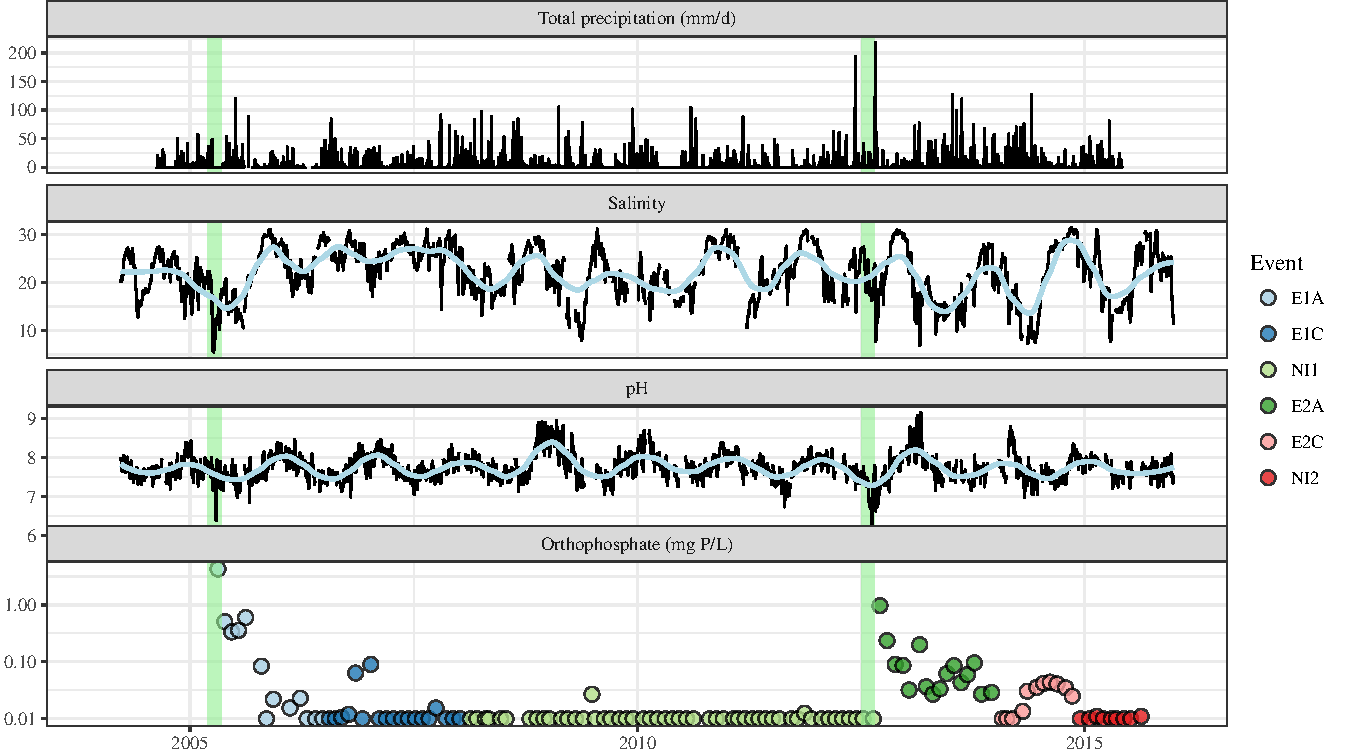
\includegraphics[width=1.3\textwidth]{figs/Fig2} 

}

\caption[Time series of total precipitation, salinity, pH, and phosphate for Bangs Lake, Grand Bay reserve]{Time series of total precipitation, salinity, pH, and phosphate for Bangs Lake, Grand Bay reserve.  All observations are daily averages, excluding phosphate which was sampled monthly.  Vertical green bars indicate a heavy rain event in April 2005 and hurricane Isaac in August 2012.  Salinity and pH include a loess smooth to reduce variability. Orthophosphate is colored by event categories in relation to the vertical green bars.  E1A: event 1 acute, E1C: event 1 chronic, NI1: non-impact 1, E2A: event 2 acute, E2C: event 2 chronic, and NI2: non-impact 2.}\label{fig:Fig2}
\end{figure}


\end{landscape}
\clearpage

\begin{figure}[!ht]

{\centering 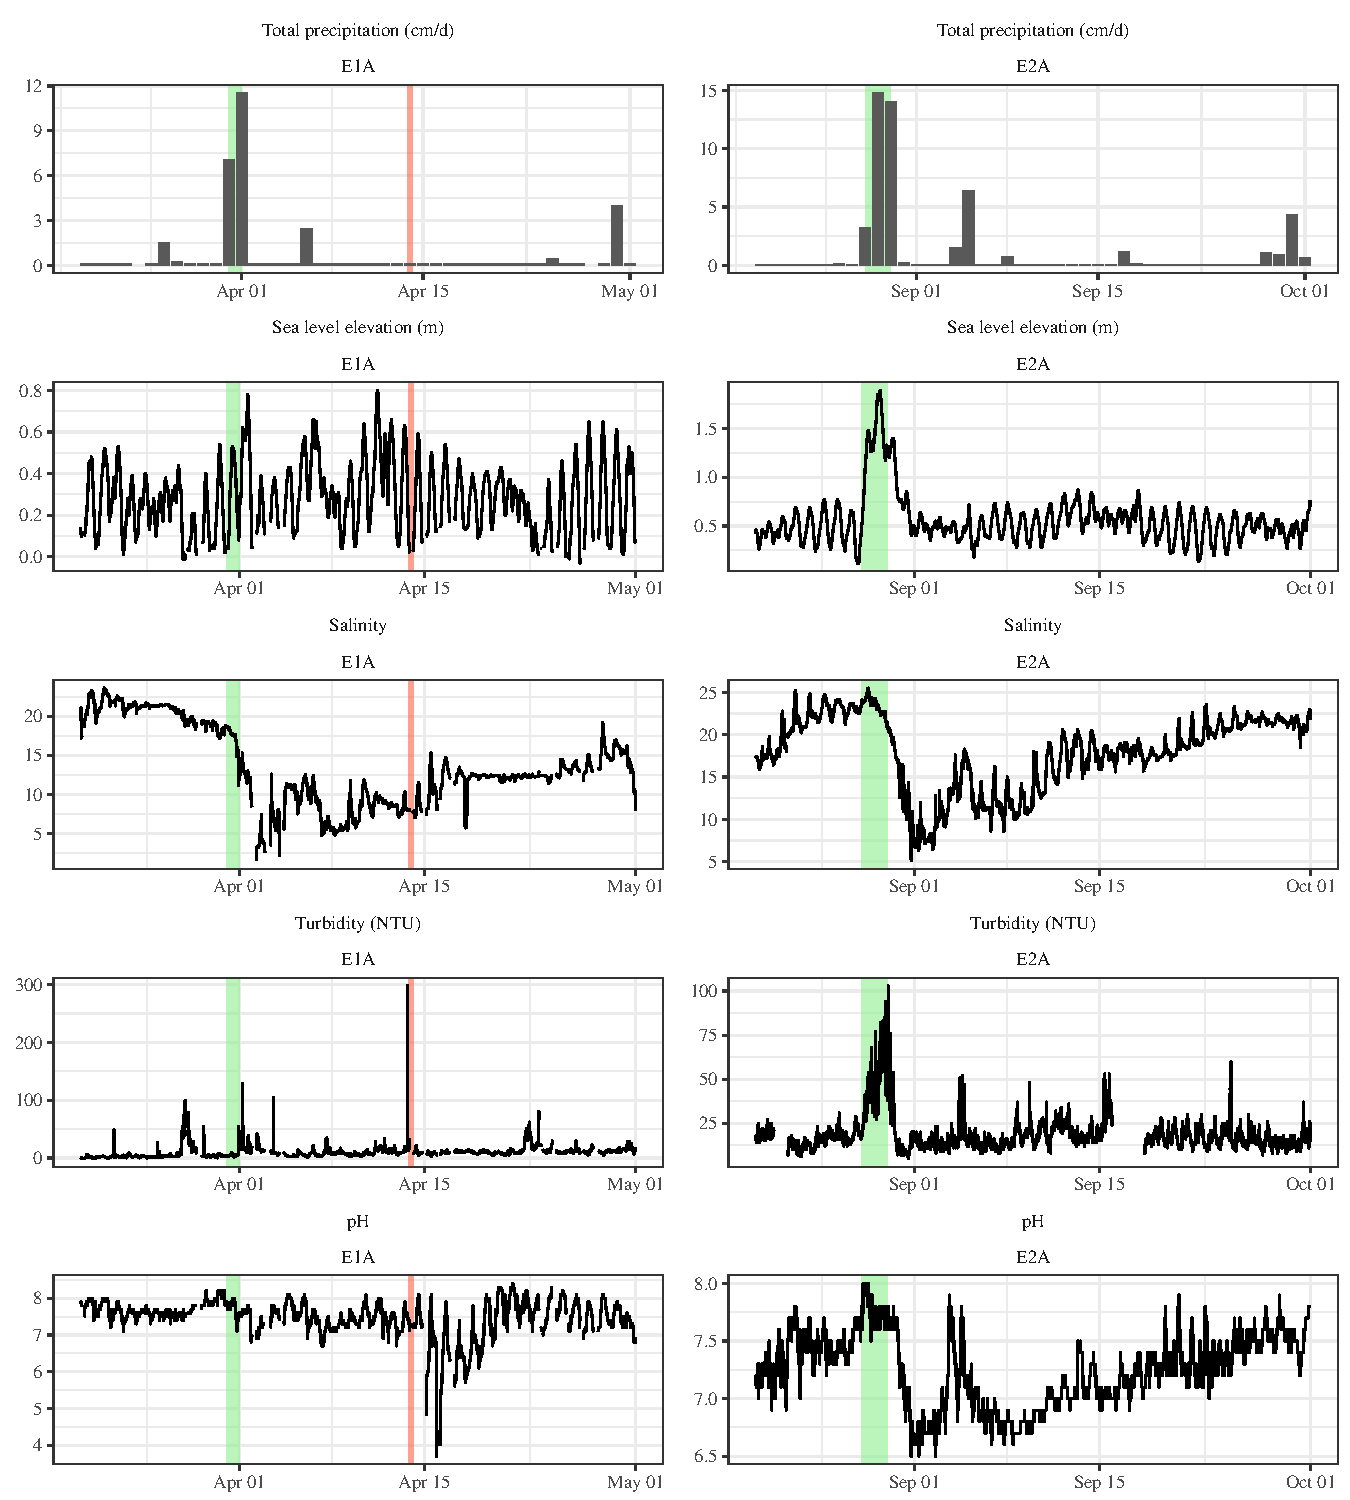
\includegraphics[width=\maxwidth]{figs/Fig3} 

}

\caption[Time series of daily precipitation, salinity, and pH for Bangs Lake, Grand Bay reserve]{Time series of daily precipitation, salinity, and pH for Bangs Lake, Grand Bay reserve.  Precipitation data are daily totals from the Pascagoula International Airport.  Salinity and pH data were collected at 15 minute time steps.  Green shading indicates period of high precipitation for a heavy rain event in 2005 (left, March 31\textsuperscript{st} to April 1\textsuperscript{st}) and hurricane Isaac in 2012 (right, August 28\textsuperscript{th} to 30\textsuperscript{th}).  Red shading for the first event indicates the date of documented phosphorus spill.  E1A: event 1 acute, E2A: event 2 acute.}\label{fig:Fig3}
\end{figure}


\clearpage

\begin{figure}[!ht]

{\centering 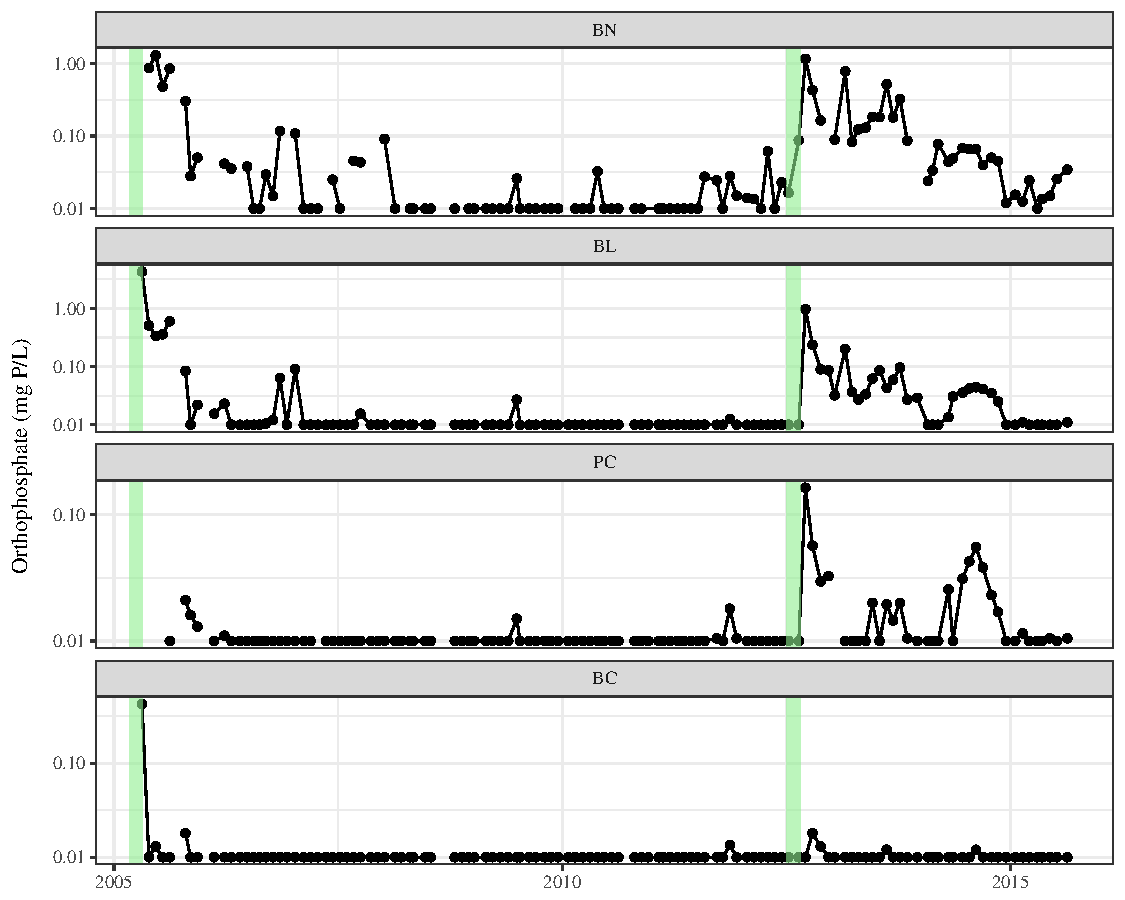
\includegraphics[width=\maxwidth]{figs/Fig4} 

}

\caption[Monthly phosphate time series at Bangs North (BN), Bangs Lake (BL), Point aux Chenes (PC), and Bayou Cumbest (BC) sites at Grand Bay]{Monthly phosphate time series at Bangs North (BN), Bangs Lake (BL), Point aux Chenes (PC), and Bayou Cumbest (BC) sites at Grand Bay. Vertical green bars indicate a heavy rain event in April 2005 and hurricane Isaac in August 2012.}\label{fig:Fig4}
\end{figure}


\clearpage

\begin{figure}[!ht]

{\centering 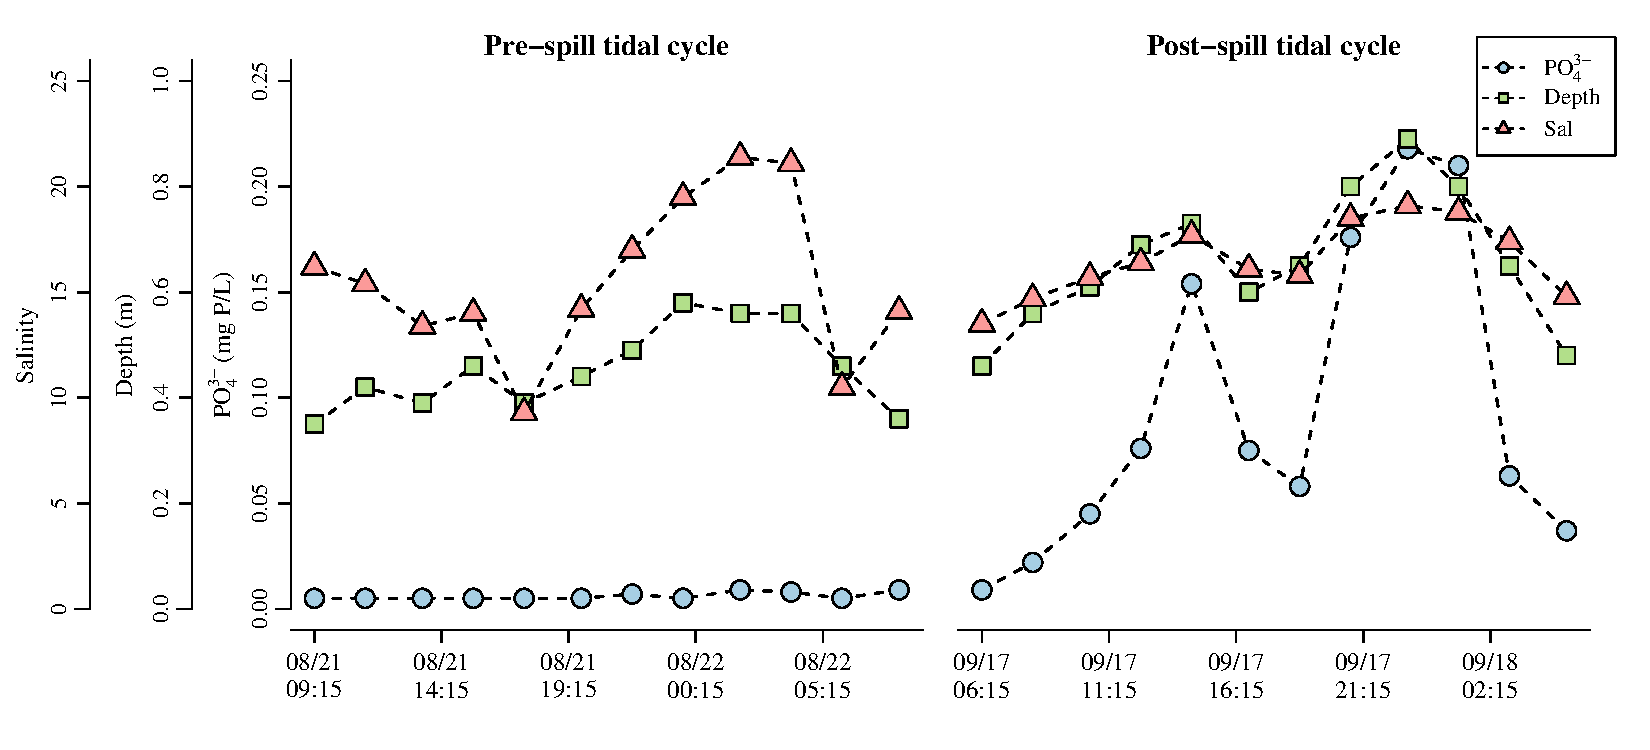
\includegraphics[width=\maxwidth]{figs/Fig5} 

}

\caption{Boxplot summaries by event of monthly orthophosphate data at Bangs Lake (BL), Bangs North (BN), and Point aux Chenes (PC), and Bayou Cumbest (BC) sites in Grand Bay.  Boxes represent the interquartile range (IQR, 25\textsuperscript{th} to 75\textsuperscript{th} percentile) with the median as the middle horizonal line.  Outliers are present beyond whiskers (1.5$\cdot$IQR). Boxes are shaded by medians between sites.  See \cref{tab:orthtab1} for a numerical summary. E1A: event 1 acute, E1C: event 1 chronic, NI1: non-impact 1, E2A: event 2 acute, E2C: event 2 chronic, and NI2: non-impact 2.}\label{fig:Fig5}
\end{figure}


\clearpage

% summary charactistics table
%latex.default(tab, file = "", rowlabel = "Stations", caption = cap,     caption.loc = "top", rgroup = rgrps, n.rgroup = rep(4, 7),     rowname = rows, colheads = c("Average", "Median", "St. Dev",         "Min", "Max"), label = "tab:summtab")%
\begin{table}[!tbp]
\caption{Site summaries of water quality (hourly) and nutrient (monthly) observations from 2005 to 2015.  Units are mg L$^{-1}$ for all variables, except Chl-\textit{a} as $\mu$g L$^{-1}$, pH from 0-12, and salinity as psu. Nutrient summaries are based on maximum likelihood estimates for left-censored data.  Sites are BC: Bayou Cumbest, BH: Bayou Heron (no nutrient data), BL: Bangs Lake, BN: Bangs North (no water quality data), and PC: Point aux Chenes.\label{tab:summtab}} 
\begin{center}
\begin{tabular}{lrrrrr}
\hline\hline
\multicolumn{1}{l}{Stations}&\multicolumn{1}{c}{Average}&\multicolumn{1}{c}{Median}&\multicolumn{1}{c}{St. Dev}&\multicolumn{1}{c}{Min}&\multicolumn{1}{c}{Max}\tabularnewline
\hline
{\bfseries Chl-\textit{a}}&&&&&\tabularnewline
~~BC&$10.82$&$ 6.69$&$13.76$&$0.69$&$ 47.67$\tabularnewline
~~BL&$ 8.25$&$ 5.43$&$ 9.44$&$0.46$&$ 41.98$\tabularnewline
~~BN&$ 7.94$&$ 5.01$&$ 9.79$&$0.55$&$ 36.71$\tabularnewline
~~PC&$ 7.98$&$ 5.17$&$ 9.39$&$0.52$&$ 33.95$\tabularnewline
\hline
{\bfseries DO$_{sat}$}&&&&&\tabularnewline
~~BC&$80.12$&$80.90$&$19.11$&$1.80$&$221.90$\tabularnewline
~~BH&$45.26$&$47.00$&$27.19$&$0.00$&$165.80$\tabularnewline
~~BL&$92.05$&$93.10$&$16.26$&$8.60$&$297.70$\tabularnewline
~~PC&$97.08$&$97.90$&$15.52$&$8.40$&$221.90$\tabularnewline
\hline
{\bfseries NH$_4^+$}&&&&&\tabularnewline
~~BC&$ 0.04$&$ 0.01$&$ 0.08$&$0.01$&$  0.21$\tabularnewline
~~BL&$ 0.02$&$ 0.01$&$ 0.06$&$0.01$&$  0.18$\tabularnewline
~~BN&$ 0.03$&$ 0.01$&$ 0.07$&$0.01$&$  0.16$\tabularnewline
~~PC&$ 0.02$&$ 0.01$&$ 0.06$&$0.01$&$  0.42$\tabularnewline
\hline
{\bfseries NO$_2^-$/NO$_3^{2-}$}&&&&&\tabularnewline
~~BC&$ 0.01$&$ 0.01$&$ 0.02$&$0.01$&$  0.09$\tabularnewline
~~BL&$ 0.01$&$ 0.00$&$ 0.03$&$0.01$&$  0.09$\tabularnewline
~~BN&$ 0.01$&$ 0.00$&$ 0.02$&$0.01$&$  0.10$\tabularnewline
~~PC&$ 0.01$&$ 0.00$&$ 0.04$&$0.01$&$  0.10$\tabularnewline
\hline
{\bfseries pH}&&&&&\tabularnewline
~~BC&$ 7.26$&$ 7.30$&$ 0.46$&$5.10$&$  9.00$\tabularnewline
~~BH&$ 6.88$&$ 7.00$&$ 0.64$&$4.00$&$  8.40$\tabularnewline
~~BL&$ 7.75$&$ 7.70$&$ 0.37$&$3.70$&$  9.60$\tabularnewline
~~PC&$ 8.06$&$ 8.10$&$ 0.22$&$7.00$&$  9.00$\tabularnewline
\hline
{\bfseries PO$_4^{3-}$}&&&&&\tabularnewline
~~BC&$ 0.00$&$ 0.00$&$ 0.03$&$0.01$&$  0.43$\tabularnewline
~~BL&$ 0.09$&$ 0.00$&$ 2.13$&$0.01$&$  4.29$\tabularnewline
~~BN&$ 0.12$&$ 0.02$&$ 0.90$&$0.01$&$  1.29$\tabularnewline
~~PC&$ 0.01$&$ 0.00$&$ 0.02$&$0.01$&$  0.16$\tabularnewline
\hline
{\bfseries Salinity}&&&&&\tabularnewline
~~BC&$17.22$&$18.00$&$ 7.86$&$0.00$&$ 33.50$\tabularnewline
~~BH&$17.93$&$19.50$&$ 7.50$&$0.00$&$ 32.40$\tabularnewline
~~BL&$22.02$&$22.40$&$ 5.49$&$1.50$&$ 32.10$\tabularnewline
~~PC&$23.30$&$24.30$&$ 5.37$&$4.30$&$ 33.20$\tabularnewline
\hline
\end{tabular}\end{center}
\end{table}



% within site eval
%latex.default(tab, file = "", rowlabel = "Site", caption = cap,     caption.loc = "top", rgroup = unique(res$StationCode), n.rgroup = rep(6,         4), rowname = rows, colheads = c("Result", "n", "Median",         "Min", "Max"), label = "tab:orthtab1")%
\begin{table}[!tbp]
\caption{Within site comparisons  of monthly orthophosphate data for each time frame at Grand Bay.  Values are within-group summaries of sample size, median, and ranges for orthophosphate by station and time frame.  Result letters indicate time frames within each station that were not significantly different based on multiple comparisons with Mann-Whitney rank sum tests.  P-values were adjusted using the sequential Bonferroni method to reduce the probability of Type I errors. Sites are BC: Bayou Cumbest, BL: Bangs Lake, BN: Bangs North, and PC: Point aux Chenes.  Time frames are E1A: event 1 acute, E1C: event 1 chronic, NI1: non-impact 1, E2A: event 2 acute, E2C: event 2 chronic, and NI2: non-impact 2.\label{tab:orthtab1}} 
\begin{center}
\begin{tabular}{llrrrr}
\hline\hline
\multicolumn{1}{l}{Site}&\multicolumn{1}{c}{Result}&\multicolumn{1}{c}{n}&\multicolumn{1}{c}{Median}&\multicolumn{1}{c}{Min}&\multicolumn{1}{c}{Max}\tabularnewline
\hline
{\bfseries BL}&&&&&\tabularnewline
~~E1A&ab&$13$&$0.02$&$0.01$&$4.29$\tabularnewline
~~E1C&c&$19$&$0.01$&$0.01$&$0.09$\tabularnewline
~~NI1&d&$52$&$0.01$&$0.01$&$0.03$\tabularnewline
~~E2A&a&$16$&$0.06$&$0.03$&$0.97$\tabularnewline
~~E2C&bc&$11$&$0.03$&$0.01$&$0.04$\tabularnewline
~~NI2&bcd&$ 9$&$0.01$&$0.01$&$0.01$\tabularnewline
\hline
{\bfseries BN}&&&&&\tabularnewline
~~E1A&ab&$10$&$0.18$&$0.03$&$1.29$\tabularnewline
~~E1C&cd&$14$&$0.02$&$0.01$&$0.12$\tabularnewline
~~NI1&e&$48$&$0.01$&$0.01$&$0.09$\tabularnewline
~~E2A&a&$14$&$0.18$&$0.08$&$1.16$\tabularnewline
~~E2C&bc&$11$&$0.05$&$0.02$&$0.08$\tabularnewline
~~NI2&d&$ 9$&$0.02$&$0.01$&$0.03$\tabularnewline
\hline
{\bfseries PC}&&&&&\tabularnewline
~~E1A&a&$ 9$&$0.01$&$0.01$&$0.02$\tabularnewline
~~E1C&b&$18$&$0.01$&$0.01$&$0.01$\tabularnewline
~~NI1&b&$52$&$0.01$&$0.01$&$0.02$\tabularnewline
~~E2A&a&$15$&$0.01$&$0.01$&$0.16$\tabularnewline
~~E2C&a&$11$&$0.02$&$0.01$&$0.06$\tabularnewline
~~NI2&ab&$ 9$&$0.01$&$0.01$&$0.01$\tabularnewline
\hline
{\bfseries BC}&&&&&\tabularnewline
~~E1A&a&$13$&$0.01$&$0.01$&$0.43$\tabularnewline
~~E1C&a&$19$&$0.01$&$0.01$&$0.01$\tabularnewline
~~NI1&a&$52$&$0.01$&$0.01$&$0.01$\tabularnewline
~~E2A&a&$16$&$0.01$&$0.01$&$0.02$\tabularnewline
~~E2C&a&$11$&$0.01$&$0.01$&$0.01$\tabularnewline
~~NI2&a&$ 9$&$0.01$&$0.01$&$0.01$\tabularnewline
\hline
\end{tabular}\end{center}
\end{table}

\clearpage

% between site eval
%latex.default(tab, file = "", rowlabel = "Site", caption = cap,     caption.loc = "top", rgroup = unique(res$TimeFrame), n.rgroup = rep(4,         6), rowname = rows, colheads = c("Result", "n", "Median",         "Min", "Max"), label = "tab:orthtab2")%
\begin{table}[!tbp]
\caption{Within time frame comparisons of monthly orthophosphate data at Grand Bay.  Values are within-group summaries of sample size, median, and ranges for orthophosphate by time frame and station.  Result letters indicate stations within each time frame that were not significantly different based on multiple comparisons with Mann-Whitney rank sum tests.  P-values were adjusted using the sequential Bonferroni method to reduce the probability of Type I errors. Sites are BC: Bayou Cumbest, BL: Bangs Lake, BN: Bangs North, and PC: Point aux Chenes.  Time frames are E1A: event 1 acute, E1C: event 1 chronic, NI1: non-impact 1, E2A: event 2 acute, E2C: event 2 chronic, and NI2: non-impact 2.\label{tab:orthtab2}} 
\begin{center}
\begin{tabular}{llrrrr}
\hline\hline
\multicolumn{1}{l}{Site}&\multicolumn{1}{c}{Result}&\multicolumn{1}{c}{n}&\multicolumn{1}{c}{Median}&\multicolumn{1}{c}{Min}&\multicolumn{1}{c}{Max}\tabularnewline
\hline
{\bfseries E1A}&&&&&\tabularnewline
~~BL&bc&$13$&$0.02$&$0.01$&$4.29$\tabularnewline
~~BN&b&$10$&$0.18$&$0.03$&$1.29$\tabularnewline
~~PC&ac&$ 9$&$0.01$&$0.01$&$0.02$\tabularnewline
~~BC&a&$13$&$0.01$&$0.01$&$0.43$\tabularnewline
\hline
{\bfseries E1C}&&&&&\tabularnewline
~~BL&ab&$19$&$0.01$&$0.01$&$0.09$\tabularnewline
~~BN&b&$14$&$0.02$&$0.01$&$0.12$\tabularnewline
~~PC&a&$18$&$0.01$&$0.01$&$0.01$\tabularnewline
~~BC&a&$19$&$0.01$&$0.01$&$0.01$\tabularnewline
\hline
{\bfseries NI1}&&&&&\tabularnewline
~~BL&a&$52$&$0.01$&$0.01$&$0.03$\tabularnewline
~~BN&b&$48$&$0.01$&$0.01$&$0.09$\tabularnewline
~~PC&a&$52$&$0.01$&$0.01$&$0.02$\tabularnewline
~~BC&a&$52$&$0.01$&$0.01$&$0.01$\tabularnewline
\hline
{\bfseries E2A}&&&&&\tabularnewline
~~BL&b&$16$&$0.06$&$0.03$&$0.97$\tabularnewline
~~BN&c&$14$&$0.18$&$0.08$&$1.16$\tabularnewline
~~PC&d&$15$&$0.01$&$0.01$&$0.16$\tabularnewline
~~BC&a&$16$&$0.01$&$0.01$&$0.02$\tabularnewline
\hline
{\bfseries E2C}&&&&&\tabularnewline
~~BL&b&$11$&$0.03$&$0.01$&$0.04$\tabularnewline
~~BN&c&$11$&$0.05$&$0.02$&$0.08$\tabularnewline
~~PC&b&$11$&$0.02$&$0.01$&$0.06$\tabularnewline
~~BC&a&$11$&$0.01$&$0.01$&$0.01$\tabularnewline
\hline
{\bfseries NI2}&&&&&\tabularnewline
~~BL&a&$ 9$&$0.01$&$0.01$&$0.01$\tabularnewline
~~BN&b&$ 9$&$0.02$&$0.01$&$0.03$\tabularnewline
~~PC&a&$ 9$&$0.01$&$0.01$&$0.01$\tabularnewline
~~BC&a&$ 9$&$0.01$&$0.01$&$0.01$\tabularnewline
\hline
\end{tabular}\end{center}
\end{table}

\clearpage

% supplements
\beginsupplement

\begin{figure}[!ht]

{\centering 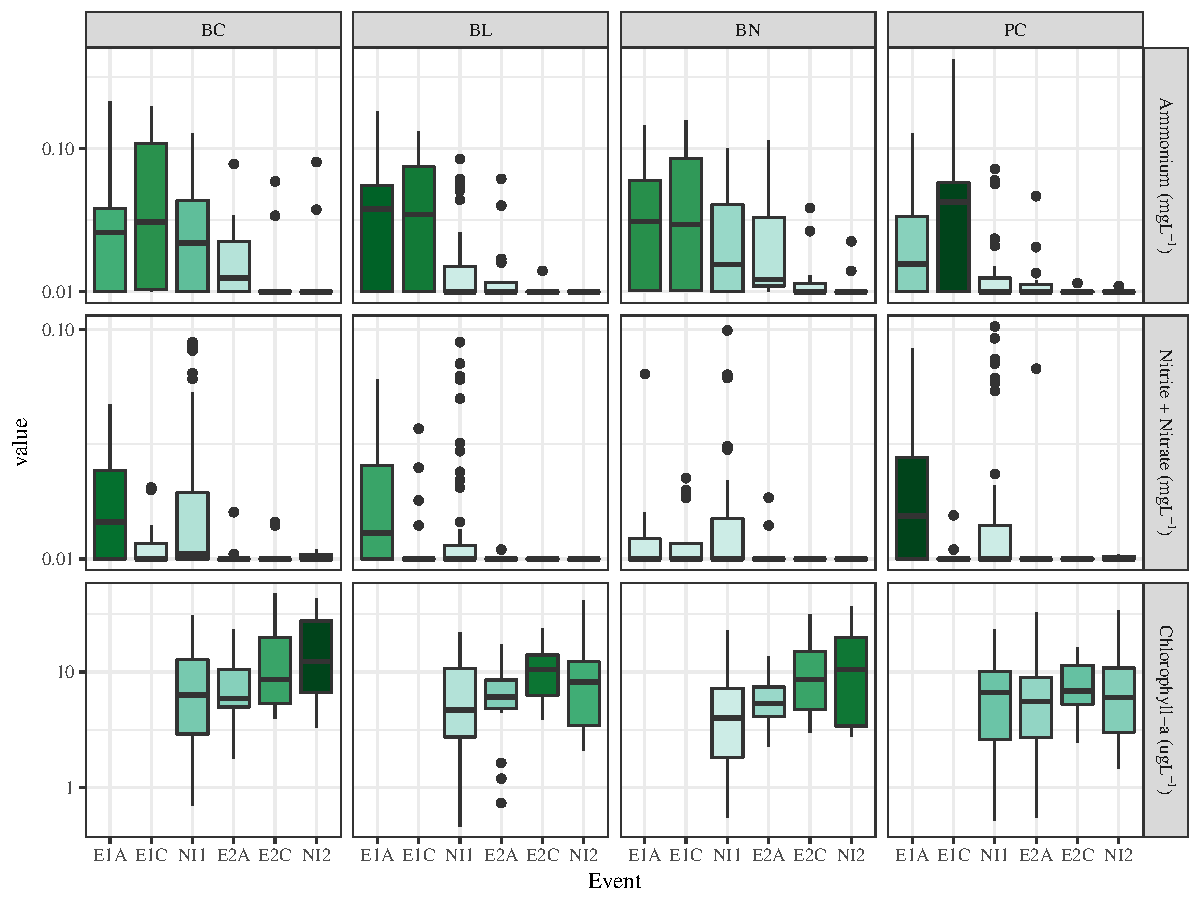
\includegraphics[width=\maxwidth]{figs/FigS1} 

}

\caption{Boxplot summaries by event of nutrient data at Bayou Cumbest (BC), Bangs Lake (BL), Bangs North (BN), and Point aux Chenes (PC) sites at Grand Bay.  Boxes represent the interquartile range (IQR, 25\textsuperscript{th} to 75\textsuperscript{th} percentile) with the median as the middle horizontal line.  Boxes are colored by relative median nutrients between sites.  Outliers are present beyond whiskers (1.5$\cdot$IQR). See \cref{tab:ammontab,tab:tntab,tab:chltab} for numerical summaries.  Insufficient chlorophyll data were removed for E1A and E1C. E1A: event 1 acute, E1C: event 1 chronic, NI1: non-impact 1, E2A: event 2 acute, E2C: event 2 chronic, and NI2: non-impact 2.}\label{fig:FigS1}
\end{figure}


\clearpage

%latex.default(tab, file = "", rowlabel = "Site", caption = cap,     caption.loc = "top", rgroup = unique(res$StationCode), n.rgroup = rep(6,         4), rowname = rows, colheads = c("Result", "n", "Median",         "Min", "Max"), label = "tab:ammontab")%
\begin{table}[!tbp]
\caption{Within site comparisons  of monthly ammonium data for each time frame at Grand Bay.  Values are within-group summaries of sample size, median, and ranges for ammonium by station and time frame.  Result letters indicate time frames within each station that were not significantly different based on multiple comparisons with Mann-Whitney rank sum tests.  P-values were adjusted using the sequential Bonferroni method to reduce the probability of Type I errors. Sites are BC: Bayou Cumbest, BL: Bangs Lake, BN: Bangs North, and PC: Point aux Chenes.  Time frames are E1A: event 1 acute, E1C: event 1 chronic, NI1: non-impact 1, E2A: event 2 acute, E2C: event 2 chronic, and NI2: non-impact 2.\label{tab:ammontab}} 
\begin{center}
\begin{tabular}{llrrrr}
\hline\hline
\multicolumn{1}{l}{Site}&\multicolumn{1}{c}{Result}&\multicolumn{1}{c}{n}&\multicolumn{1}{c}{Median}&\multicolumn{1}{c}{Min}&\multicolumn{1}{c}{Max}\tabularnewline
\hline
{\bfseries BL}&&&&&\tabularnewline
~~E1A&ab&$12$&$0.04$&$0.01$&$0.18$\tabularnewline
~~E1C&a&$18$&$0.03$&$0.01$&$0.13$\tabularnewline
~~NI1&ab&$49$&$0.01$&$0.01$&$0.08$\tabularnewline
~~E2A&ab&$16$&$0.01$&$0.01$&$0.06$\tabularnewline
~~E2C&b&$11$&$0.01$&$0.01$&$0.01$\tabularnewline
~~NI2&b&$ 9$&$0.01$&$0.01$&$0.01$\tabularnewline
\hline
{\bfseries BN}&&&&&\tabularnewline
~~E1A&a&$11$&$0.03$&$0.01$&$0.14$\tabularnewline
~~E1C&a&$15$&$0.03$&$0.01$&$0.16$\tabularnewline
~~NI1&a&$45$&$0.02$&$0.01$&$0.10$\tabularnewline
~~E2A&a&$14$&$0.01$&$0.01$&$0.11$\tabularnewline
~~E2C&a&$11$&$0.01$&$0.01$&$0.04$\tabularnewline
~~NI2&a&$ 9$&$0.01$&$0.01$&$0.02$\tabularnewline
\hline
{\bfseries PC}&&&&&\tabularnewline
~~E1A&ab&$ 8$&$0.02$&$0.01$&$0.13$\tabularnewline
~~E1C&a&$17$&$0.04$&$0.01$&$0.42$\tabularnewline
~~NI1&b&$49$&$0.01$&$0.01$&$0.07$\tabularnewline
~~E2A&ab&$16$&$0.01$&$0.01$&$0.05$\tabularnewline
~~E2C&b&$11$&$0.01$&$0.01$&$0.01$\tabularnewline
~~NI2&b&$ 9$&$0.01$&$0.01$&$0.01$\tabularnewline
\hline
{\bfseries BC}&&&&&\tabularnewline
~~E1A&a&$12$&$0.03$&$0.01$&$0.21$\tabularnewline
~~E1C&a&$18$&$0.03$&$0.01$&$0.20$\tabularnewline
~~NI1&a&$49$&$0.02$&$0.01$&$0.13$\tabularnewline
~~E2A&a&$16$&$0.01$&$0.01$&$0.08$\tabularnewline
~~E2C&a&$11$&$0.01$&$0.01$&$0.06$\tabularnewline
~~NI2&a&$ 9$&$0.01$&$0.01$&$0.08$\tabularnewline
\hline
\end{tabular}\end{center}
\end{table}

\clearpage

% between site eval
%latex.default(tab, file = "", rowlabel = "Site", caption = cap,     caption.loc = "top", rgroup = unique(res$TimeFrame), n.rgroup = rep(4,         6), rowname = rows, colheads = c("Result", "n", "Median",         "Min", "Max"), label = "tab:ammontab2")%
\begin{table}[!tbp]
\caption{Within time frame comparisons of monthly ammonium data at Grand Bay.  Values are within-group summaries of sample size, median, and ranges for ammonium by time frame and station.  Result letters indicate stations within each time frame that were not significantly different based on multiple comparisons with Mann-Whitney rank sum tests.  P-values were adjusted using the sequential Bonferroni method to reduce the probability of Type I errors. Sites are BC: Bayou Cumbest, BL: Bangs Lake, BN: Bangs North, and PC: Point aux Chenes.  Time frames are E1A: event 1 acute, E1C: event 1 chronic, NI1: non-impact 1, E2A: event 2 acute, E2C: event 2 chronic, and NI2: non-impact 2.\label{tab:ammontab2}} 
\begin{center}
\begin{tabular}{llrrrr}
\hline\hline
\multicolumn{1}{l}{Site}&\multicolumn{1}{c}{Result}&\multicolumn{1}{c}{n}&\multicolumn{1}{c}{Median}&\multicolumn{1}{c}{Min}&\multicolumn{1}{c}{Max}\tabularnewline
\hline
{\bfseries E1A}&&&&&\tabularnewline
~~BL&a&$12$&$0.04$&$0.01$&$0.18$\tabularnewline
~~BN&a&$11$&$0.03$&$0.01$&$0.14$\tabularnewline
~~PC&a&$ 8$&$0.02$&$0.01$&$0.13$\tabularnewline
~~BC&a&$12$&$0.03$&$0.01$&$0.21$\tabularnewline
\hline
{\bfseries E1C}&&&&&\tabularnewline
~~BL&a&$18$&$0.03$&$0.01$&$0.13$\tabularnewline
~~BN&a&$15$&$0.03$&$0.01$&$0.16$\tabularnewline
~~PC&a&$17$&$0.04$&$0.01$&$0.42$\tabularnewline
~~BC&a&$18$&$0.03$&$0.01$&$0.20$\tabularnewline
\hline
{\bfseries NI1}&&&&&\tabularnewline
~~BL&b&$49$&$0.01$&$0.01$&$0.08$\tabularnewline
~~BN&a&$45$&$0.02$&$0.01$&$0.10$\tabularnewline
~~PC&b&$49$&$0.01$&$0.01$&$0.07$\tabularnewline
~~BC&a&$49$&$0.02$&$0.01$&$0.13$\tabularnewline
\hline
{\bfseries E2A}&&&&&\tabularnewline
~~BL&a&$16$&$0.01$&$0.01$&$0.06$\tabularnewline
~~BN&a&$14$&$0.01$&$0.01$&$0.11$\tabularnewline
~~PC&a&$16$&$0.01$&$0.01$&$0.05$\tabularnewline
~~BC&a&$16$&$0.01$&$0.01$&$0.08$\tabularnewline
\hline
{\bfseries E2C}&&&&&\tabularnewline
~~BL&a&$11$&$0.01$&$0.01$&$0.01$\tabularnewline
~~BN&a&$11$&$0.01$&$0.01$&$0.04$\tabularnewline
~~PC&a&$11$&$0.01$&$0.01$&$0.01$\tabularnewline
~~BC&a&$11$&$0.01$&$0.01$&$0.06$\tabularnewline
\hline
{\bfseries NI2}&&&&&\tabularnewline
~~BL&a&$ 9$&$0.01$&$0.01$&$0.01$\tabularnewline
~~BN&a&$ 9$&$0.01$&$0.01$&$0.02$\tabularnewline
~~PC&a&$ 9$&$0.01$&$0.01$&$0.01$\tabularnewline
~~BC&a&$ 9$&$0.01$&$0.01$&$0.08$\tabularnewline
\hline
\end{tabular}\end{center}
\end{table}

\clearpage

%latex.default(tab, file = "", rowlabel = "Site", caption = cap,     caption.loc = "top", rgroup = unique(res$StationCode), n.rgroup = rep(6,         4), rowname = rows, colheads = c("Result", "n", "Median",         "Min", "Max"), label = "tab:tntab")%
\begin{table}[!tbp]
\caption{Within site comparisons  of monthly nitrogen (nitrate, nitrite) data for each time frame at Grand Bay.  Values are within-group summaries of sample size, median, and ranges for nitrogen by station and time frame.  Result letters indicate time frames within each station that were not significantly different based on multiple comparisons with Mann-Whitney rank sum tests.  P-values were adjusted using the sequential Bonferroni method to reduce the probability of Type I errors. Sites are BC: Bayou Cumbest, BL: Bangs Lake, BN: Bangs North, and PC: Point aux Chenes.  Time frames are E1A: event 1 acute, E1C: event 1 chronic, NI1: non-impact 1, E2A: event 2 acute, E2C: event 2 chronic, and NI2: non-impact 2.\label{tab:tntab}} 
\begin{center}
\begin{tabular}{llrrrr}
\hline\hline
\multicolumn{1}{l}{Site}&\multicolumn{1}{c}{Result}&\multicolumn{1}{c}{n}&\multicolumn{1}{c}{Median}&\multicolumn{1}{c}{Min}&\multicolumn{1}{c}{Max}\tabularnewline
\hline
{\bfseries BL}&&&&&\tabularnewline
~~E1A&a&$14$&$0.01$&$0.01$&$0.06$\tabularnewline
~~E1C&ab&$19$&$0.01$&$0.01$&$0.04$\tabularnewline
~~NI1&ab&$53$&$0.01$&$0.01$&$0.09$\tabularnewline
~~E2A&b&$15$&$0.01$&$0.01$&$0.01$\tabularnewline
~~E2C&ab&$11$&$0.01$&$0.01$&$0.01$\tabularnewline
~~NI2&ab&$ 3$&$0.01$&$0.01$&$0.01$\tabularnewline
\hline
{\bfseries BN}&&&&&\tabularnewline
~~E1A&a&$11$&$0.01$&$0.01$&$0.06$\tabularnewline
~~E1C&a&$16$&$0.01$&$0.01$&$0.02$\tabularnewline
~~NI1&a&$49$&$0.01$&$0.01$&$0.10$\tabularnewline
~~E2A&a&$13$&$0.01$&$0.01$&$0.02$\tabularnewline
~~E2C&a&$11$&$0.01$&$0.01$&$0.01$\tabularnewline
~~NI2&a&$ 3$&$0.01$&$0.01$&$0.01$\tabularnewline
\hline
{\bfseries PC}&&&&&\tabularnewline
~~E1A&a&$10$&$0.02$&$0.01$&$0.08$\tabularnewline
~~E1C&a&$18$&$0.01$&$0.01$&$0.02$\tabularnewline
~~NI1&a&$53$&$0.01$&$0.01$&$0.10$\tabularnewline
~~E2A&a&$15$&$0.01$&$0.01$&$0.07$\tabularnewline
~~E2C&a&$11$&$0.01$&$0.01$&$0.01$\tabularnewline
~~NI2&a&$ 3$&$0.01$&$0.01$&$0.01$\tabularnewline
\hline
{\bfseries BC}&&&&&\tabularnewline
~~E1A&a&$14$&$0.01$&$0.01$&$0.05$\tabularnewline
~~E1C&ab&$19$&$0.01$&$0.01$&$0.02$\tabularnewline
~~NI1&ab&$53$&$0.01$&$0.01$&$0.09$\tabularnewline
~~E2A&b&$16$&$0.01$&$0.01$&$0.02$\tabularnewline
~~E2C&ab&$11$&$0.01$&$0.01$&$0.01$\tabularnewline
~~NI2&ab&$ 3$&$0.01$&$0.01$&$0.01$\tabularnewline
\hline
\end{tabular}\end{center}
\end{table}

\clearpage

% between site eval
%latex.default(tab, file = "", rowlabel = "Site", caption = cap,     caption.loc = "top", rgroup = unique(res$TimeFrame), n.rgroup = rep(4,         6), rowname = rows, colheads = c("Result", "n", "Median",         "Min", "Max"), label = "tab:tntab2")%
\begin{table}[!tbp]
\caption{Within time frame comparisons of monthly nitrogen (nitrate, nitrite) data at Grand Bay.  Values are within-group summaries of sample size, median, and ranges for nitrogen by time frame and station.  Result letters indicate stations within each time frame that were not significantly different based on multiple comparisons with Mann-Whitney rank sum tests.  P-values were adjusted using the sequential Bonferroni method to reduce the probability of Type I errors. Sites are BC: Bayou Cumbest, BL: Bangs Lake, BN: Bangs North, and PC: Point aux Chenes.  Time frames are E1A: event 1 acute, E1C: event 1 chronic, NI1: non-impact 1, E2A: event 2 acute, E2C: event 2 chronic, and NI2: non-impact 2.\label{tab:tntab2}} 
\begin{center}
\begin{tabular}{llrrrr}
\hline\hline
\multicolumn{1}{l}{Site}&\multicolumn{1}{c}{Result}&\multicolumn{1}{c}{n}&\multicolumn{1}{c}{Median}&\multicolumn{1}{c}{Min}&\multicolumn{1}{c}{Max}\tabularnewline
\hline
{\bfseries E1A}&&&&&\tabularnewline
~~BL&a&$14$&$0.01$&$0.01$&$0.06$\tabularnewline
~~BN&a&$11$&$0.01$&$0.01$&$0.06$\tabularnewline
~~PC&a&$10$&$0.02$&$0.01$&$0.08$\tabularnewline
~~BC&a&$14$&$0.01$&$0.01$&$0.05$\tabularnewline
\hline
{\bfseries E1C}&&&&&\tabularnewline
~~BL&a&$19$&$0.01$&$0.01$&$0.04$\tabularnewline
~~BN&a&$16$&$0.01$&$0.01$&$0.02$\tabularnewline
~~PC&a&$18$&$0.01$&$0.01$&$0.02$\tabularnewline
~~BC&a&$19$&$0.01$&$0.01$&$0.02$\tabularnewline
\hline
{\bfseries NI1}&&&&&\tabularnewline
~~BL&a&$53$&$0.01$&$0.01$&$0.09$\tabularnewline
~~BN&a&$49$&$0.01$&$0.01$&$0.10$\tabularnewline
~~PC&a&$53$&$0.01$&$0.01$&$0.10$\tabularnewline
~~BC&a&$53$&$0.01$&$0.01$&$0.09$\tabularnewline
\hline
{\bfseries E2A}&&&&&\tabularnewline
~~BL&a&$15$&$0.01$&$0.01$&$0.01$\tabularnewline
~~BN&a&$13$&$0.01$&$0.01$&$0.02$\tabularnewline
~~PC&a&$15$&$0.01$&$0.01$&$0.07$\tabularnewline
~~BC&a&$16$&$0.01$&$0.01$&$0.02$\tabularnewline
\hline
{\bfseries E2C}&&&&&\tabularnewline
~~BL&a&$11$&$0.01$&$0.01$&$0.01$\tabularnewline
~~BN&a&$11$&$0.01$&$0.01$&$0.01$\tabularnewline
~~PC&a&$11$&$0.01$&$0.01$&$0.01$\tabularnewline
~~BC&a&$11$&$0.01$&$0.01$&$0.01$\tabularnewline
\hline
{\bfseries NI2}&&&&&\tabularnewline
~~BL&a&$ 3$&$0.01$&$0.01$&$0.01$\tabularnewline
~~BN&a&$ 3$&$0.01$&$0.01$&$0.01$\tabularnewline
~~PC&a&$ 3$&$0.01$&$0.01$&$0.01$\tabularnewline
~~BC&a&$ 3$&$0.01$&$0.01$&$0.01$\tabularnewline
\hline
\end{tabular}\end{center}
\end{table}

\clearpage

%latex.default(tab, file = "", rowlabel = "Site", caption = cap,     caption.loc = "top", rgroup = unique(res$StationCode), n.rgroup = rep(4,         4), rowname = rows, colheads = c("Result", "n", "Median",         "Min", "Max"), label = "tab:chltab")%
\begin{table}[!tbp]
\caption{Within site comparisons  of monthly chlorophyll data for each time frame at Grand Bay.  Values are within-group summaries of sample size, median, and ranges for chlorophyll by station and time frame.  Result letters indicate time frames within each station that were not significantly different based on multiple comparisons with Mann-Whitney rank sum tests.  P-values were adjusted using the sequential Bonferroni method to reduce the probability of Type I errors. Sites are BC: Bayou Cumbest, BL: Bangs Lake, BN: Bangs North, and PC: Point aux Chenes.  Time frames are NI1: non-impact 1, E2A: event 2 acute, E2C: event 2 chronic, and NI2: non-impact 2.\label{tab:chltab}} 
\begin{center}
\begin{tabular}{llrrrr}
\hline\hline
\multicolumn{1}{l}{Site}&\multicolumn{1}{c}{Result}&\multicolumn{1}{c}{n}&\multicolumn{1}{c}{Median}&\multicolumn{1}{c}{Min}&\multicolumn{1}{c}{Max}\tabularnewline
\hline
{\bfseries BL}&&&&&\tabularnewline
~~NI1&a&$54$&$ 4.66$&$0.46$&$21.99$\tabularnewline
~~E2A&a&$16$&$ 6.05$&$0.73$&$17.28$\tabularnewline
~~E2C&a&$11$&$10.56$&$3.90$&$23.89$\tabularnewline
~~NI2&a&$ 9$&$ 8.21$&$2.10$&$41.98$\tabularnewline
\hline
{\bfseries BN}&&&&&\tabularnewline
~~NI1&a&$50$&$ 3.98$&$0.55$&$23.05$\tabularnewline
~~E2A&a&$14$&$ 5.37$&$2.26$&$13.71$\tabularnewline
~~E2C&a&$11$&$ 8.56$&$3.02$&$31.29$\tabularnewline
~~NI2&a&$ 9$&$10.47$&$2.78$&$36.71$\tabularnewline
\hline
{\bfseries PC}&&&&&\tabularnewline
~~NI1&a&$54$&$ 6.63$&$0.52$&$23.39$\tabularnewline
~~E2A&a&$16$&$ 5.57$&$0.55$&$32.52$\tabularnewline
~~E2C&a&$11$&$ 6.81$&$2.44$&$16.46$\tabularnewline
~~NI2&a&$ 9$&$ 6.00$&$1.47$&$33.95$\tabularnewline
\hline
{\bfseries BC}&&&&&\tabularnewline
~~NI1&a&$54$&$ 6.34$&$0.69$&$30.59$\tabularnewline
~~E2A&a&$16$&$ 5.91$&$1.78$&$23.12$\tabularnewline
~~E2C&a&$11$&$ 8.57$&$3.93$&$47.67$\tabularnewline
~~NI2&a&$ 9$&$12.35$&$3.33$&$43.42$\tabularnewline
\hline
\end{tabular}\end{center}
\end{table}

\clearpage

% between site eval
%latex.default(tab, file = "", rowlabel = "Site", caption = cap,     caption.loc = "top", rgroup = unique(res$TimeFrame), n.rgroup = rep(4,         4), rowname = rows, colheads = c("Result", "n", "Median",         "Min", "Max"), label = "tab:chltab2")%
\begin{table}[!tbp]
\caption{Within time frame comparisons of monthly chlorophyll data at Grand Bay.  Values are within-group summaries of sample size, median, and ranges for chlorophyll by time frame and station.  Result letters indicate stations within each time frame that were not significantly different based on multiple comparisons with Mann-Whitney rank sum tests.  P-values were adjusted using the sequential Bonferroni method to reduce the probability of Type I errors. Sites are BC: Bayou Cumbest, BL: Bangs Lake, BN: Bangs North, and PC: Point aux Chenes.  Time frames are NI1: non-impact 1, E2A: event 2 acute, E2C: event 2 chronic, and NI2: non-impact 2.\label{tab:chltab2}} 
\begin{center}
\begin{tabular}{llrrrr}
\hline\hline
\multicolumn{1}{l}{Site}&\multicolumn{1}{c}{Result}&\multicolumn{1}{c}{n}&\multicolumn{1}{c}{Median}&\multicolumn{1}{c}{Min}&\multicolumn{1}{c}{Max}\tabularnewline
\hline
{\bfseries NI1}&&&&&\tabularnewline
~~BL&a&$54$&$ 4.66$&$0.46$&$21.99$\tabularnewline
~~BN&a&$50$&$ 3.98$&$0.55$&$23.05$\tabularnewline
~~PC&a&$54$&$ 6.63$&$0.52$&$23.39$\tabularnewline
~~BC&a&$54$&$ 6.34$&$0.69$&$30.59$\tabularnewline
\hline
{\bfseries E2A}&&&&&\tabularnewline
~~BL&a&$16$&$ 6.05$&$0.73$&$17.28$\tabularnewline
~~BN&a&$14$&$ 5.37$&$2.26$&$13.71$\tabularnewline
~~PC&a&$16$&$ 5.57$&$0.55$&$32.52$\tabularnewline
~~BC&a&$16$&$ 5.91$&$1.78$&$23.12$\tabularnewline
\hline
{\bfseries E2C}&&&&&\tabularnewline
~~BL&a&$11$&$10.56$&$3.90$&$23.89$\tabularnewline
~~BN&a&$11$&$ 8.56$&$3.02$&$31.29$\tabularnewline
~~PC&a&$11$&$ 6.81$&$2.44$&$16.46$\tabularnewline
~~BC&a&$11$&$ 8.57$&$3.93$&$47.67$\tabularnewline
\hline
{\bfseries NI2}&&&&&\tabularnewline
~~BL&a&$ 9$&$ 8.21$&$2.10$&$41.98$\tabularnewline
~~BN&a&$ 9$&$10.47$&$2.78$&$36.71$\tabularnewline
~~PC&a&$ 9$&$ 6.00$&$1.47$&$33.95$\tabularnewline
~~BC&a&$ 9$&$12.35$&$3.33$&$43.42$\tabularnewline
\hline
\end{tabular}\end{center}
\end{table}

\clearpage

\end{document}
